\chapter{Identifying and Validating the Environment Model }

Physiological models are developed to represent certain clinical conditions common across a population of patients, or the condition of a specific patient. Consequently, the structure of the model and corresponding parameters have to be identified. This information can be obtained from electrogram data collected during medical procedures and from physiological literature in which population data has been analyzed and summarized. Due to limited interactions with the patient (e.g. during a device implantation procedure or an ablation procedure), currently the quality and quantity of patient-specific physiological data is sparse as there is generally not enough information to identify all the parameters in the model.  A model with the spatio-temporal structure that is similar to the conduction patterns in the heart helps simplify the process of identifying the model parameters. A rigorous procedure for the model identification step is an important contributor to the model validation step. In this chapter, we aim to answer the following questions:
%%It is essential to choose the right level of abstraction so that the model is identifiable (to a large extent). Having physiological correspondence for the model structure and parameters can also simplify the identification process. 

\begin{itemize}
	\vspace{-5pt}
	\item What is the importance of model identification for closed-loop simulation and model checking?
	\vspace{-5pt}
    	\item How are models identified from patient data and patient population parameters?
\end{itemize}

In the following section, we briefly discuss our model identification effort for heart models used in two closed-loop verification applications, and their corresponding challenges. This is followed by the procedures to validate the heart models before they are used for closed-loop verification and testing of the pacemaker.
\begin{figure}[!t]
\centering
		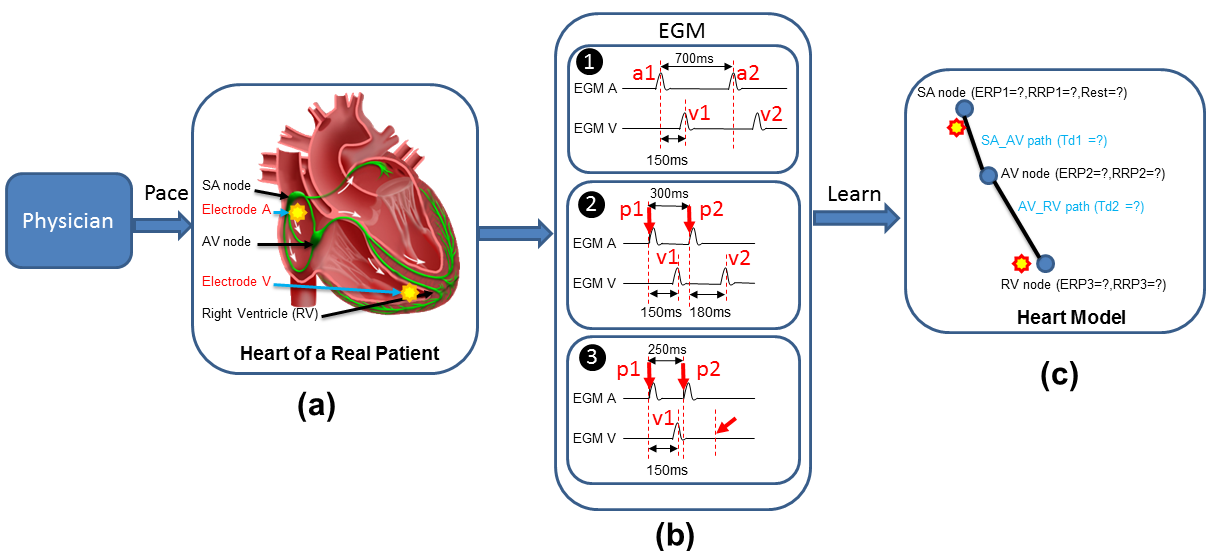
\includegraphics[width=0.9  \textwidth]{figs/modelID.png}
		
%\vspace{-10pt}
\caption{\small (a) The illustration of the probe locations. (b) Multiple pacing sequences with different timing outcomes. (c) The heart model with undecided parameters}
\label{fig:modelID}
%\vspace{-15pt}
\end{figure} 

\section{Heart Model Identification for Closed-loop Simulation}
In closed-loop simulation, a deterministic heart model should be identified to represent a specific patient under a certain heart condition. The constraints for model parameters can be obtained from patient data with \emph{Electrophysiological (EP) Testing}. During EP testing, the physician delivers electrical pacing sequences from electrodes placed inside the patient's heart to instigate responses along fast and slow conduction pathways. The observed patterns and timing of electrical events are used to extract extract conduction and propagation properties of different tissue regions across the myocardium. Since the goal for any EP testing procedure is not to determine all the timing parameters for a patient, the amount of parameters that can be identified from the patient data is limited.    

\figref{modelID} illustrates how timing parameters can be extracted during an EP testing procedure. \figref{modelID}(a) shows a setup with two electrodes placed in the right atrium and right ventricle of the heart respectively. EGM signals can be measured from these two electrodes (\figref{modelID}(b)). The physician delivers long and short interval pacing sequences through the electrodes which may trigger different responses along different conduction pathways from the patient's heart. \figref{modelID}(c) shows a heart model structure with unknown parameter values. By analyzing the \emph{timing} and \emph{pattern} of the EGM signals we extract constraints on the heart model parameters. In EGM sequence 1, the interval between two intrinsic activations $a1$ and $a2$ in EGM A is 700ms, so we have:
$$ERP1+RRP1+Rest=700ms$$
The interval between $a1$ and $v1$ is 150ms, so we have:
$$Td1+Td2=150ms$$
In EGM sequence 2, the pacing interval from Electrode A is 300ms. By observing that the interval between $p1-v1$ is less than the interval between $p2-v2$, we know that $p2$ arrives during the RRP period of the AV node. So we have:
$$ERP1+RRP1\leq 300ms$$
In EGM sequence 3, the pacing interval is further reduced to 250ms. There is no $v2$ corresponding to $p2$, indicating $p2$ arrives during the ERP period of the AV node. So we have:
$$ERP1\leq 250ms$$
Each experiment provides additional time constraints for model parameters. By systematically conducting experiments certain model parameters can be uniquely identified within a relatively tight range. However, even with simplified model structure like the one in the example, not all model parameters can be uniquely identified due to limited number of electrodes and limited number of experiments during a real procedure.






\subsection{Heart Model Identification in Closed-loop Model Checking}
In model checking, the heart models have simpler structure and fewer parameters due to non-deterministic abstraction. The placement and connectivity of nodes and paths in the heart models are developed to be consistent with EP practice. This way, each node and path automata and their timing parameters have physiological correspondence to parameters found in literature (\figref{intervals}). The range for non-deterministic parameters directly corresponds to the range for possible values of the respective physiological parameters. Therefore, model identification for model checking is much simpler and . 

\begin{figure}[!t]
\centering
		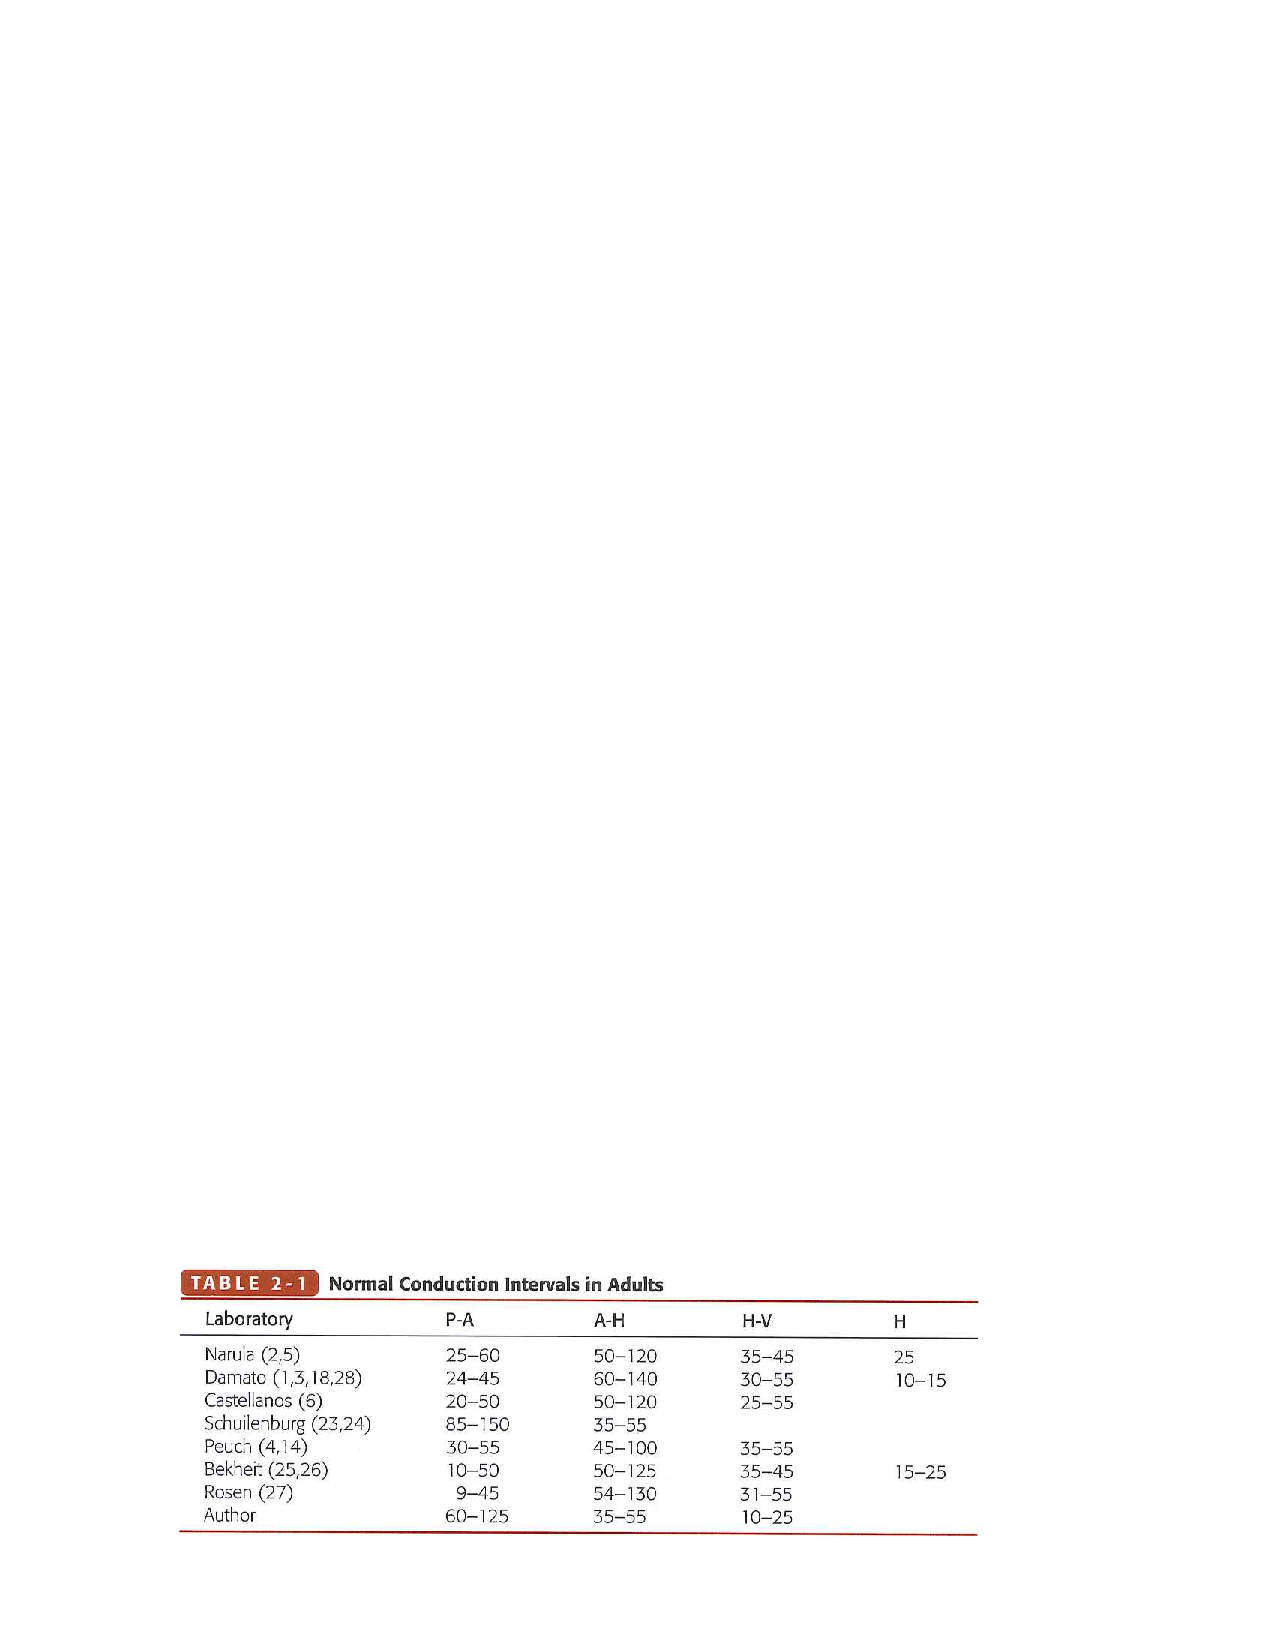
\includegraphics[width=0.8\textwidth]{figs/intervals.pdf}
		
%\vspace{-10pt}
\caption{\small Timing intervals measured during clinical studies \cite{josephson}}
\label{fig:intervals}
%\vspace{-15pt}
\end{figure} 



%%%%%%%%%%%%%%%%%%%%%%%%%%%%%%%%%%%%%
%%%%%%%%%%%%%%%%%%%%%%%%%%%%%%%%%%%%%


\section{Validating the Environment Model}
%The validity of the environment models affects the validity of the closed-loop verification results. 
Since models are approximations of the actual environment, there are always discrepancies between the model and the actual patient (group). The challenge then is to evaluate the confidence in the safety guarantees that model-based closed-loop verification can provide. The metric and process to validate the environment model is different for the two applications of heart modeling: in closed-loop model checking, the model's \textbf{coverage} on environmental behaviors is more important, while in closed-loop simulation, the \textbf{accuracy} of the model is more important. In this chapter, we aim to answer the following questions and use our heart models as examples to demonstrate different validation procedures which improve the fidelity of the environment model. 
\begin{itemize}
	\vspace{-5pt}
	\item What are the different methods to validate physiological models?
	\vspace{-5pt}
	\item How much confidence is sufficient from the model validation process?
\end{itemize}

\subsection{Validating Models for Closed-loop Simulation}
A physiological model is considered valid for closed-loop simulation if (a) it is capable of generating the same output as the patient given the same input; and (b) it is general enough to represent other patients with similar conditions by adjusting its parameters. The second point is to ensure that the model successfully captures the underlying mechanism instead of over-fitting the data. In the following example we demonstrate the capability of our heart models to model certain heart conditions according to the mechanism described in physiological literature, and the model exhibits expected output given the proposed inputs.

%To use a physiological model for closed-loop simulation, there are two levels of validity: 1) model a patient with certain heart condition, 2) model a \em ph{specific} patient with certain heart condition. Level 1 validity ensures that the model successfully models the underlying mechanism of the heart condition, while level 2 validity guarantees the capability of the model to generate same data as the corresponding patient given the same input. Note that satisfying level 2 without satisfying level 1 may result in over-fitting.
\begin{figure}[!t]
\centering
		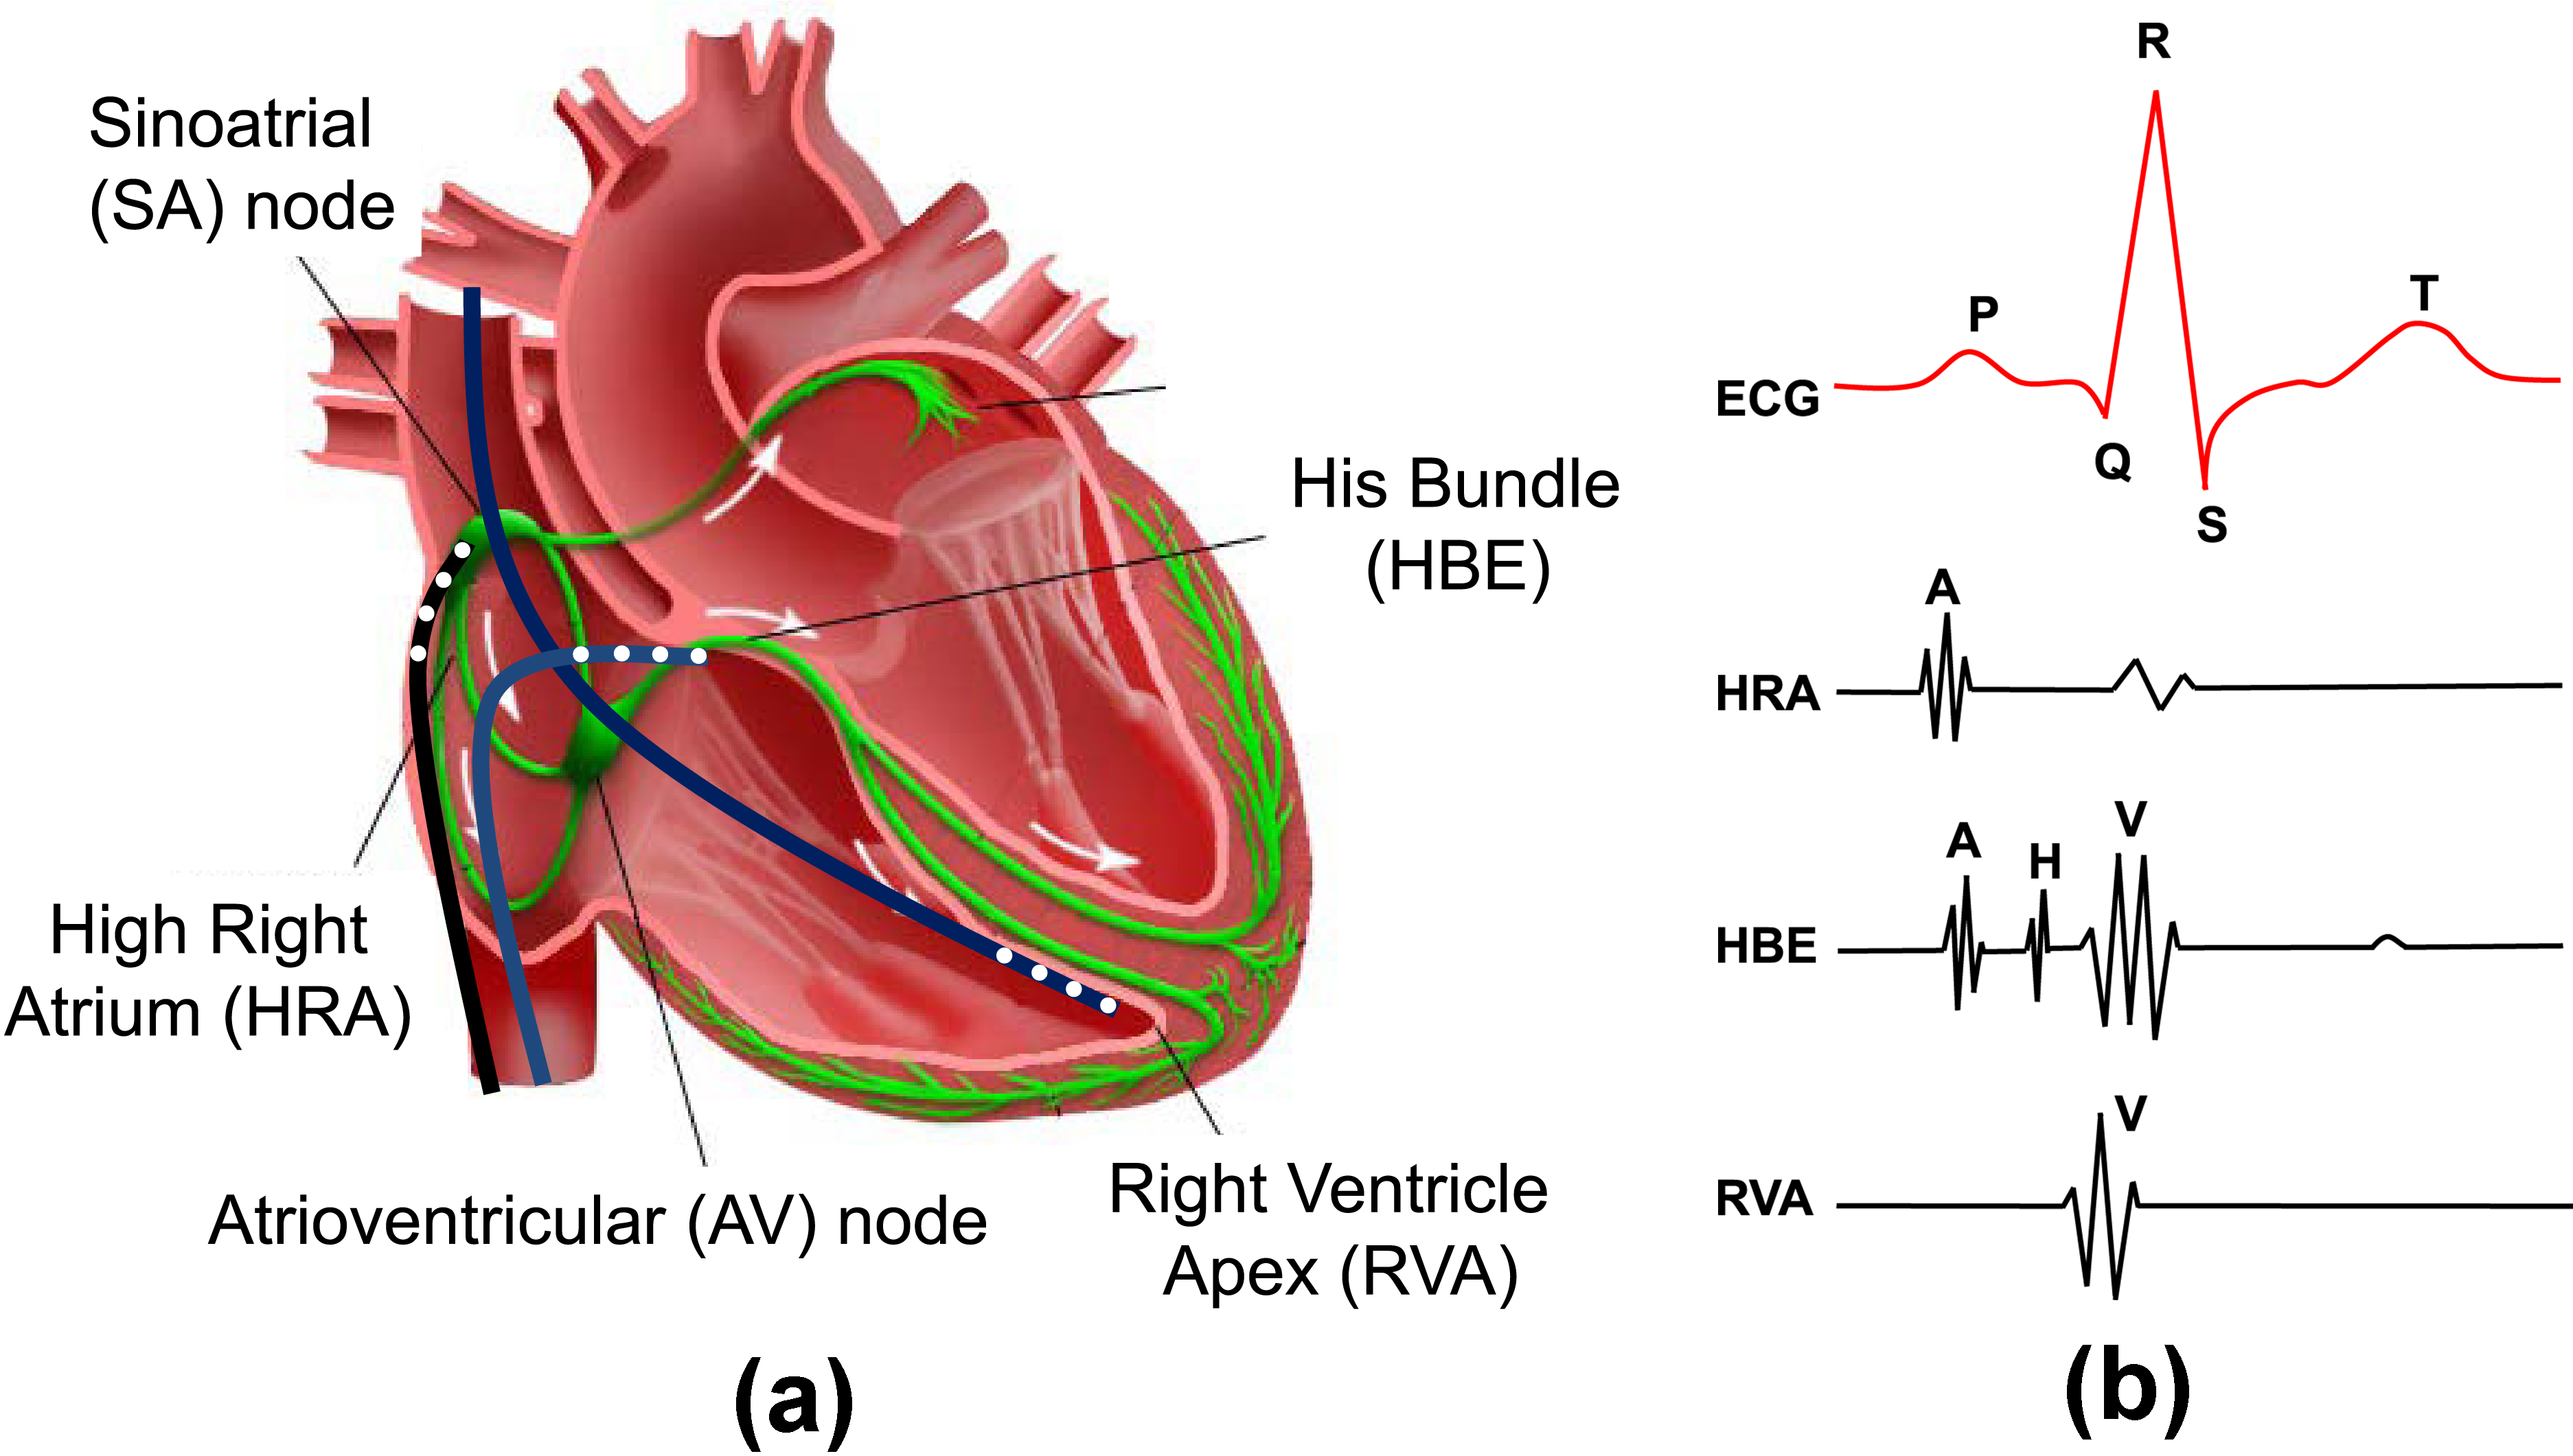
\includegraphics[width=0.9  \textwidth]{figs/probes.png}
		
%\vspace{-10pt}
\caption{\small (a) Probe locations for a general EP testing procedure. (b) EGM signals measured from the probes}
\label{fig:egm}
%\vspace{-15pt}
\end{figure} 

During an EP testing procedure, the physician place catheters inside the patient's heart to observe local electrical activities from different locations of the heart. The His bundle catheter (HBE) is particularly important when evaluating the atria-to-ventricle conduction path (\figref{egm}). For each A to V conduction there are 3 impulses which correspond to atrial contraction (A), His bundle activation (H) and ventricular activation (V).  In this case study, two pacing signals $a1$ and $a2$ are delivered to the heart from the HRA catheter. By gradually decreasing the pacing interval in each test, certain tissue along the A-V conduction path will be activated during its refractory period, thus affecting the conduction delay further down the conduction path and change the intervals between the impulses. \figref{book_1}.a shows the relation between pacing interval ($a1$-$a2$) and corresponding intervals between A, H and V impulses. On the left side it shows that interval $H_1-H_2$ and $V_1-V_2$ decrease but remain equal as the pacing interval decreases, indicating the tissue with the longest refractory period along the path is not between the His Bundle and the ventricles. When the pacing interval decreases to 350ms both intervals increases, indicating that the RRP of certain tissue has been reached and the tissue is between the atria and the His bundle. On the right it shows that the $A_2-H_2$ interval increases as the pacing interval decreases, which further proves the hypothesis that the AV node, which is between the atria and the His bundle has the longest refractory period along the A-V conduction path. We configured our heart model such that the AV node has the longest refractory period and performed the same study by decreasing the pacing interval. The result shows the exact same trend as the real patient (\figref{type_1}).
\begin{figure*}[!t]
\centering
		\subfigure 	[\small] 
		{
		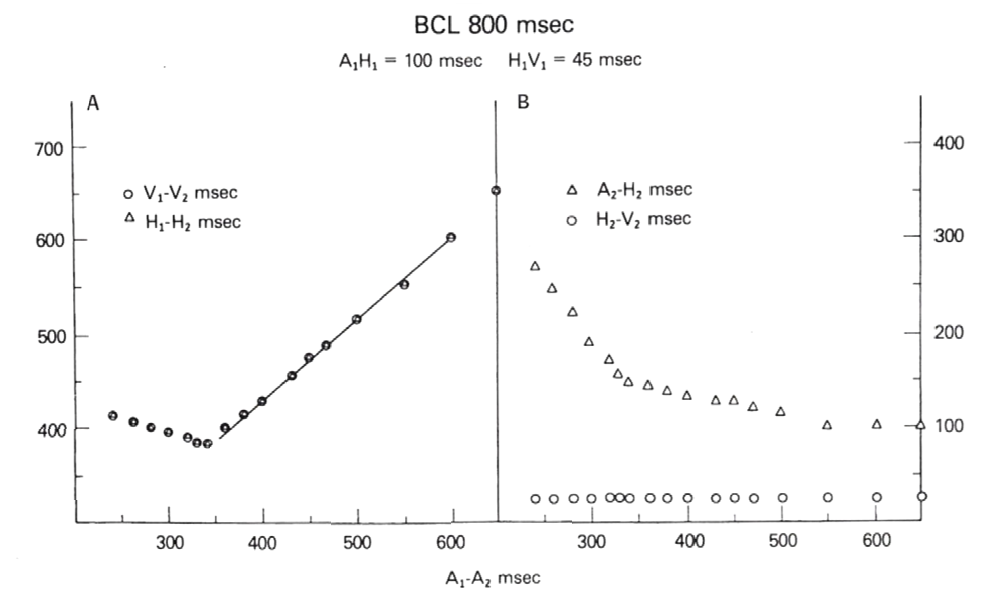
\includegraphics[width=0.5\textwidth]{figs/book_1.png}
		\label{fig:book_1}
		} 
		\subfigure [\small ] 
		{	
			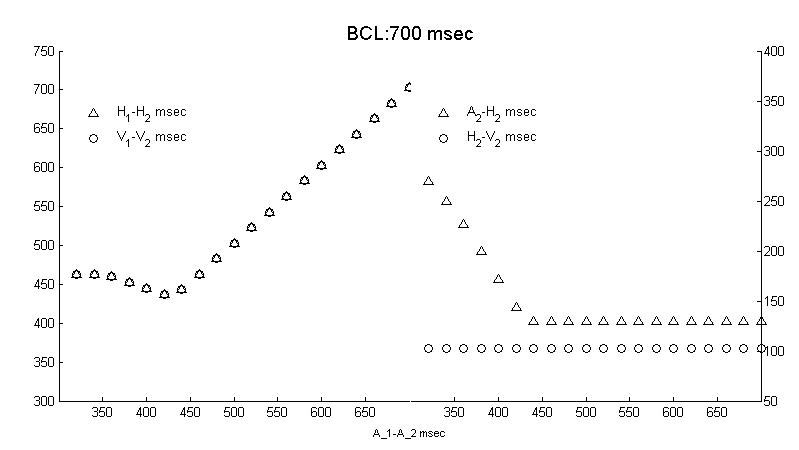
\includegraphics[width=0.45\textwidth]{figs/type_1.png} 
			\label{fig:type_1}
		}
\label{fig:Case_1}
%\vspace{-5pt}
\caption{\small Key interval values when the coupling interval shortens for (a) a real patient (\cite{josephson}) and (b) in heart model simulation (\cite{vhm_ecrts10}).}
%\vspace{-15pt}
\end{figure*} 


% \begin{figure}[\b]
% 	\center
% 	\vspace{-20pt}
% %	\includegraphics[width=0.49\textwidth]{figs/AV_reentry_circuit.pdf}
% 	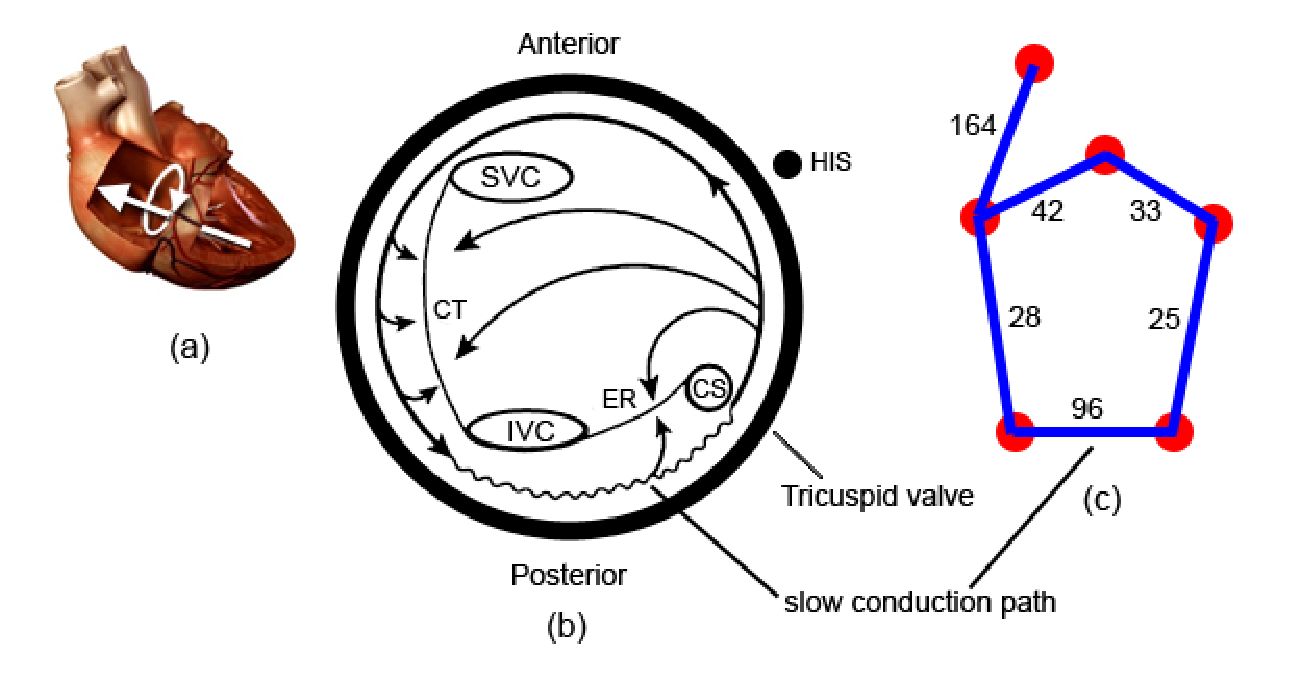
\includegraphics[width=0.5\textwidth]{figs/AFL_circuit.pdf}
% 	\center
% 	\vspace{-15pt}
% 	\caption{(a) The straight arrow shows the view of the AFL circuit from the right ventricle through the tricuspid valve into the right atrium, while the curved area shows the direction of conduction. (b) The circuit is bounded by the eustachian ridge (ER), connecting the  inferior vena cava (IVC) and the coronary sinus (CS), as well as the crista terminalis (CT), connecting the superior vena cava (SVC) and the IVC. The wavy line shows slow conduction through the CTI, bounded by the ER and the tricuspid valve (\emph{Adapted from} \cite{AFL_diag}). (c) The AFL circuit in the VHM extrapolates nodes and paths from the true physiology. The numbers show the values of conduction timers in the paths, with corresponding slow conduction path on the bottom.}
% 	\label{fig:AFL}
% \end{figure}
\begin{figure*}[!t]
\centering
		\subfigure 	[\small Electrograms of induced Wenckebach block in a
patient] 
		{
		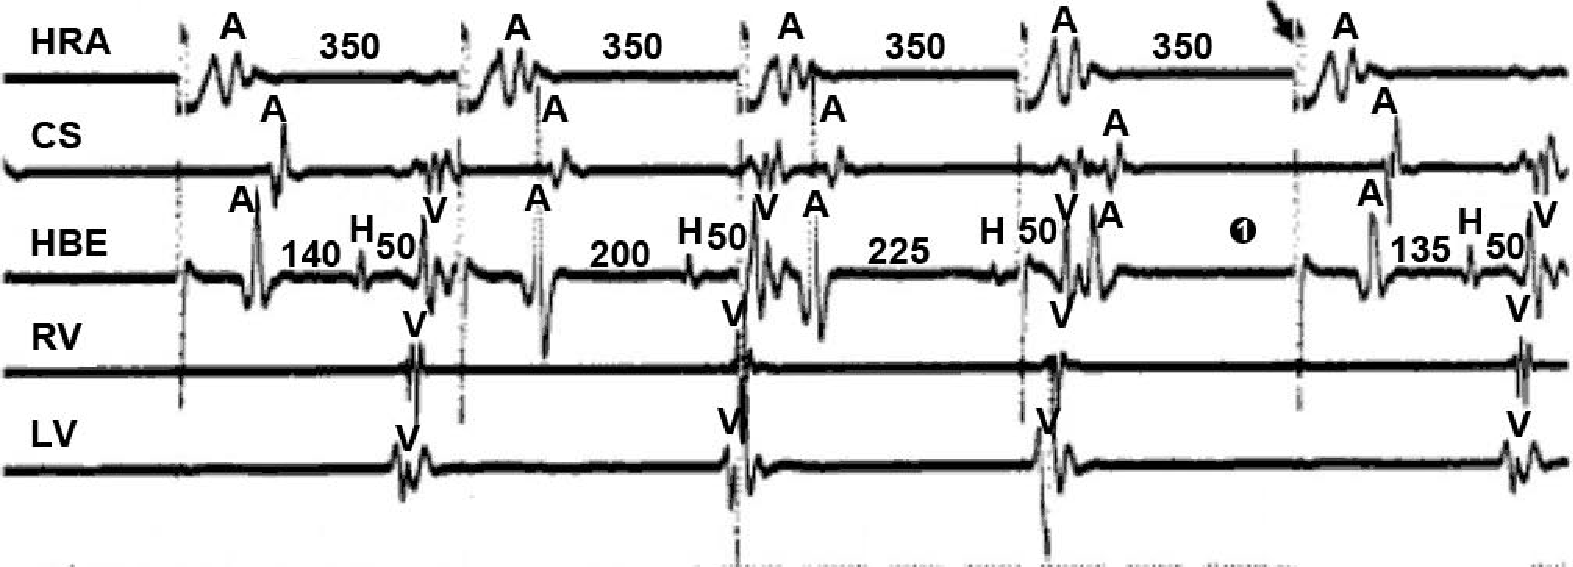
\includegraphics[width=0.40\textwidth]{figs/wenckebach_book.pdf}
		\label{fig:WB_book}
		} 
		\hspace{.1in}%
		\subfigure [\small Electrograms of induced Wenckebach block in
the heart model with BCL 420 msec] 
		{	
			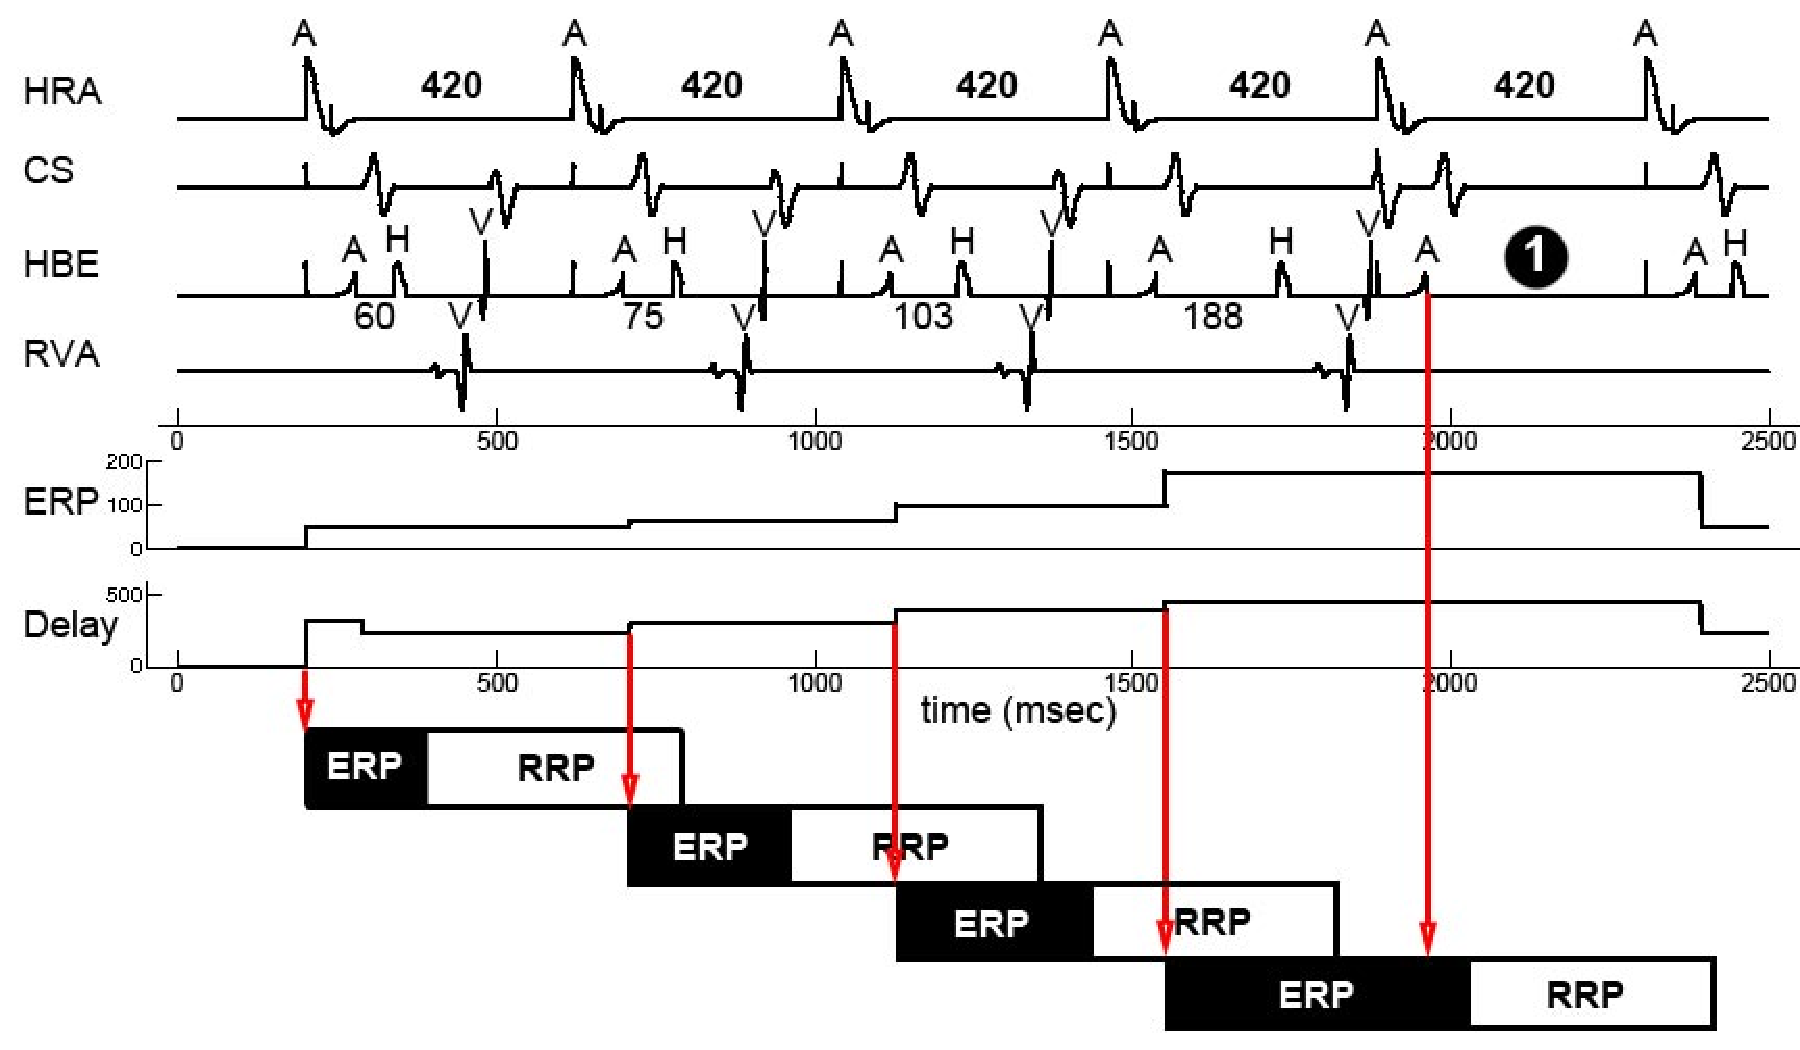
\includegraphics[width=0.40\textwidth]{figs/WB_new.pdf} 
			\label{fig:WB}
		}
\vspace{-5pt}
\caption{}
\vspace{-15pt}
\end{figure*} 
%%%%%%%%%%%%%%%%%%%%%%%%%%%%%%%%%%%%%%%%%%%%
This heart condition can also show Wenckebach type A-V nodal response. In this case, a sequence of pacing signals with a short coupling interval ($A_1-A_2<=AV.Terp+AV.Trrp$) is delivered in the atrium. This results in a gradual increase in the AV nodal conduction delay and then a dropped beat occurs in the ventricle due to the increased ERP period of the AV node. The EGMs for a real patient with Wenckebach type A-V nodal response are shown in \figref{WB_book}. With the VHM, we observe similar behavior, and the gradually increasing ERP and conduction delay are visualized in \figref{WB}.
\subsection{Validating Models for Closed-loop Model Checking}
In model checking, a lot of complex dynamics of the environment are abstracted so that the environment model covers large number of environmental behaviors using non-determinism. The validity of the model is obtained by a valid initial model and a rigorous abstraction processes. In \cite{STTT13}, we started with a valid detailed deterministic model (as described above) and by applying different abstraction steps we were able to generate a series of non-deterministic heart models. Between each abstraction step, the heart models satisfy a timed simulation relationship (\cite{simulation}) which is described below. The timed simulation guarantees all behaviors are covered in the mode abstract model.

For two timed automata $T^1=\left\langle S^1,S_0^1,\Sigma^1,X^1,inv^1,E^1\right\rangle$ and $T^2=\left\langle S^2,S_0^2,\Sigma^2,X^2,inv^2,E^2\right\rangle$, a timed simulation relation is a binary relation $\textsf{sim}\subseteq \Omega^1\times \Omega^2$ where $\Omega^1$ and $\Omega^2$ are sets of states of $T^1$ and $T^2$. We say $T^2$ \textsf{time simulates} $T^1$ ($T^1 \preceq_t T^2$) if the following conditions holds:
\begin{itemize}
	\item Initial states correspondence: $(\left\langle s_0^1,\textbf{0}\right\rangle,\left\langle s_0^2,\textbf{0}\right\rangle)\in \textsf{sim}$
	\item Timed transition: For every $(\left\langle s_1,v_1\right\rangle,\left\langle s_2,v_2\right\rangle)\in\textsf{sim}$, if $\left\langle s_1,v_1\right\rangle\xrightarrow{\delta}\left\langle s_1,v_1+\delta\right\rangle$, there exists $\left\langle s_2,v_2+\delta\right\rangle$ such that $\left\langle s_2,v_2\right\rangle\xrightarrow{\delta}\left\langle s_2,v_2+\delta\right\rangle$ and \\$(\left\langle s_1,v_1+\delta\right\rangle,\left\langle s_2,v_2+\delta\right\rangle)\in\textsf{sim}$.
	\item Discrete transition: For every $(\left\langle s_1,v_1\right\rangle,\left\langle s_2,v_2\right\rangle)\in\textsf{sim}$, if $\left\langle s_1,v_1\right\rangle\xrightarrow{\sigma}\left\langle s_1',v_1'\right\rangle$, there exists $\left\langle s_2',v_2'\right\rangle$ such that $\left\langle s_2,v_2\right\rangle\xrightarrow{\sigma}\left\langle s_2',v_2'\right\rangle$ and $(\left\langle s_1',v_1'\right\rangle,\left\langle s_2',v_2'\right\rangle)\in\textsf{sim}$.
\end{itemize}

The validated heart models can then be used for closed-loop verification of implantable pacemaker. Both the identification and validation of the heart models can be used to provide more confidence to the verification results, which would be helpful during certification process.
 